\documentclass[11pt,a4paper]{article}
\usepackage[latin5]{inputenc}
\usepackage[english]{babel}
\usepackage{amsmath}
\usepackage{amsfonts}
\usepackage{amssymb}
\usepackage{graphicx,subfig}
\usepackage{placeins}
\usepackage{gensymb}


\begin{document}

\section{Grab Cut}
Grab cut is a very elegant algorithm for image segmentation. We were asked to use it on a series of images. Luckily, OpenCV provides us with a very neat implementation of the grab cut algorithm.
\begin{figure}
\centering
\subfloat[][The original image]{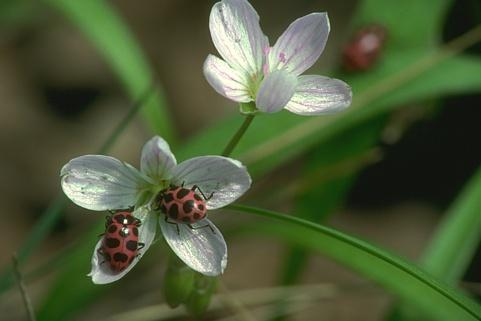
\includegraphics[scale=.3]{data/grabcut-dataset/35008.jpg}}
\quad
\subfloat[][Grab Cut]{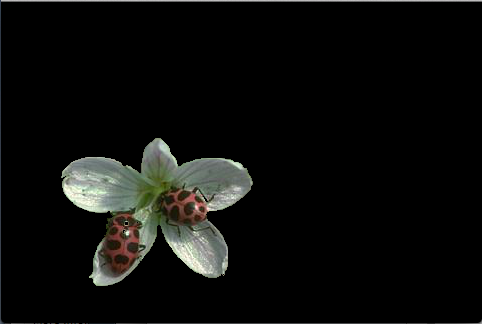
\includegraphics[scale=.3]{data/grabcut-dataset/res/marie.png}}

\caption{Grab cut on this image works very well. The petals and the bugs are extracted within 2 iterations of the algorithm. Extraction of a single bug by placing the grab rectangle around one of them is not possible (picture not shown)}%

\end{figure}

\begin{figure}
\centering
\subfloat[][The original image]{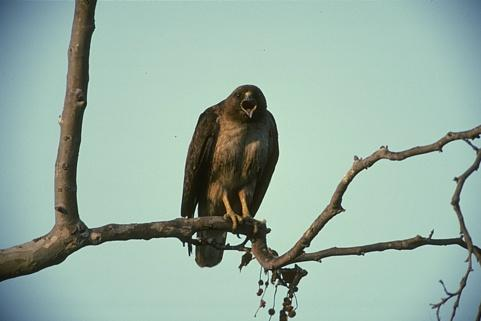
\includegraphics[scale=.3]{data/grabcut-dataset/42049.jpg}}
\quad
\subfloat[][Grab Cut]{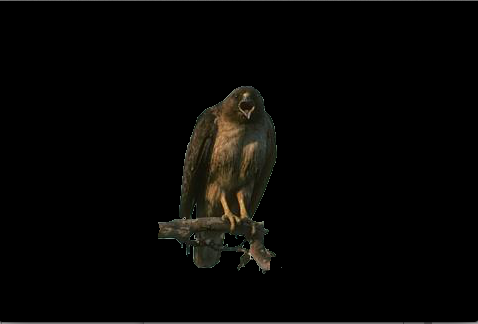
\includegraphics[scale=.3]{data/grabcut-dataset/res/eagle.png}}

\caption{The eagle is extracted quite nicely, although it takes up to 10-15 iterations until the sky parts between wing and body are recognized as background. As can be seen, it is also not possible to completely segment away the tree branch. This is not very surprising since the color of the bark is very similar to the color of the bird.}%

\end{figure}

\begin{figure}
\centering
\subfloat[][The original image]{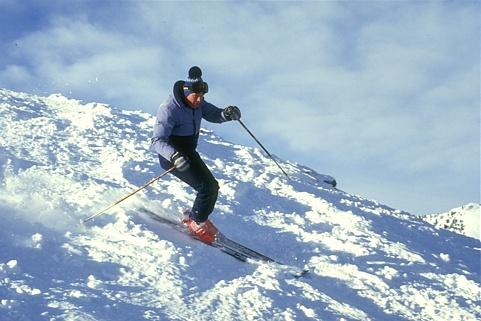
\includegraphics[scale=.3]{data/grabcut-dataset/61060.jpg}}
\quad
\subfloat[][Grab Cut big box]{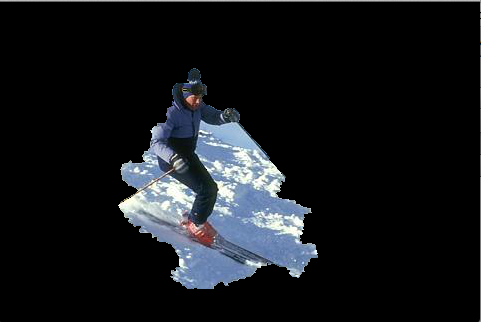
\includegraphics[scale=.3]{data/grabcut-dataset/res/skier2.png}}

\quad
\subfloat[][Grab Cut small box]{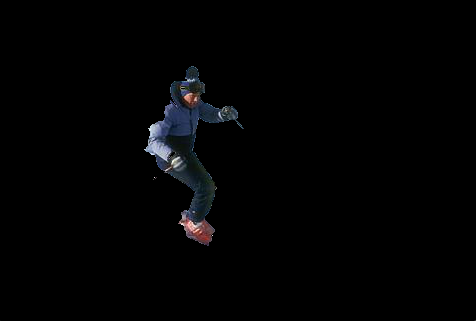
\includegraphics[scale=.3]{data/grabcut-dataset/res/skier3.png}}

\quad
\subfloat[][Grab Cut small box]{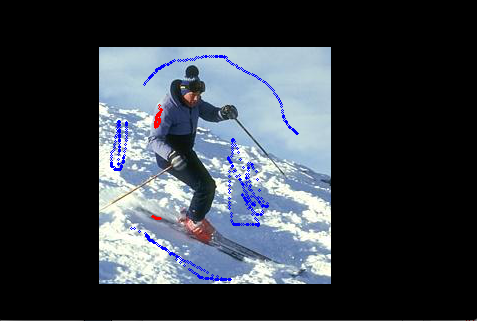
\includegraphics[scale=.3]{data/grabcut-dataset/res/skier4.png}}

\quad
\subfloat[][Grab Cut small box]{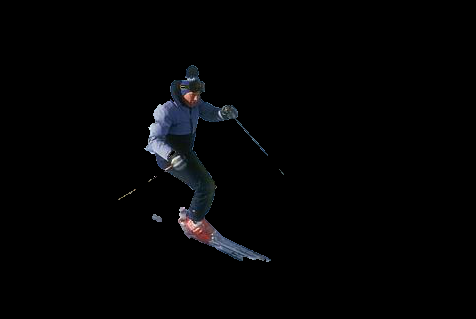
\includegraphics[scale=.3]{data/grabcut-dataset/res/skier5.png}}


\caption{This image proves to be tricky to segment. When the bounding rectangle is drawin around the whole skier (including skies), the resulting segmentation stabilizes after around 10 iterations with b), which clearly is not usable. When the rectangle is only drawn around the body, it also takes around 10 iterations to result in c), which is a little better, but now lacks part of the skier. In d) the grab cut algorithm is provided with additional background and foreground pixels, the result in d) is obtained after around 5 iterations.}%

\end{figure}

\begin{figure}
\centering
\subfloat[][The original image]{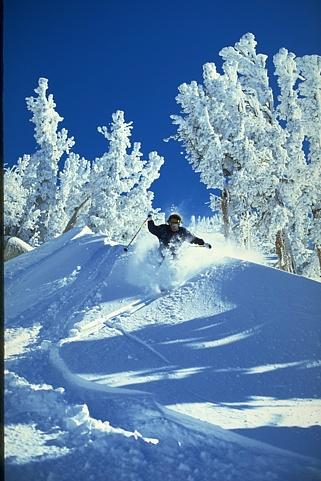
\includegraphics[scale=.3]{data/grabcut-dataset/225017.jpg}}
\quad
\subfloat[][Grab Cut]{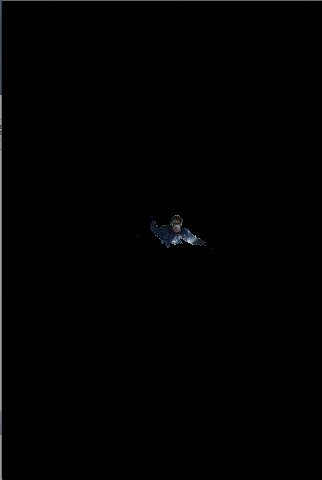
\includegraphics[scale=.3]{data/grabcut-dataset/res/skier6.png}}

\caption{Clear segmentation of this image proves hard again. This is probably due to the fact that the object of interest, the skier, is partly hidden behind a cloud of snow.}%

\end{figure}

\begin{figure}
\centering
\subfloat[][The original image]{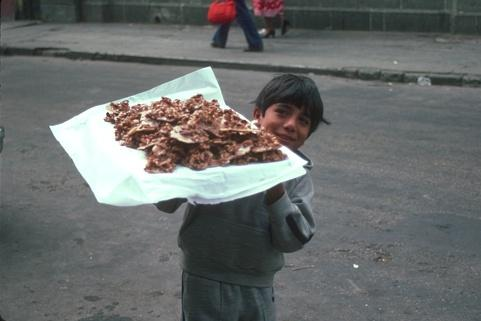
\includegraphics[scale=.3]{data/grabcut-dataset/90076.jpg}}
\quad
\subfloat[][Grab Cut]{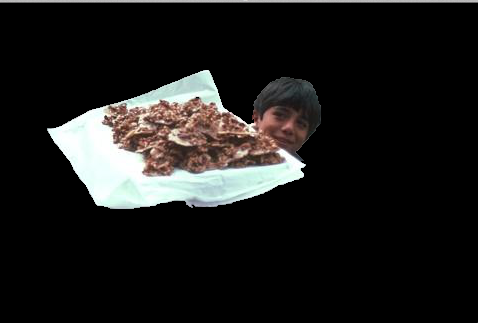
\includegraphics[scale=.3]{data/grabcut-dataset/res/kid.png}}

\caption{Clear segmentation of this image proves hard again. This is because the pants and sweather of the kid are gray, similar to the color of the street. Better results could be achieved by marking additional foreground pixels (data not shown).}%

\end{figure}

\begin{figure}
\centering
\subfloat[][The original image]{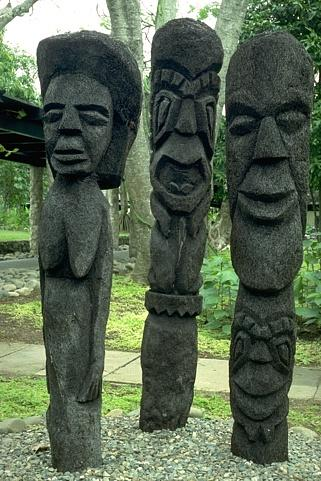
\includegraphics[scale=.3]{data/grabcut-dataset/101085.jpg}}
\quad
\subfloat[][Grab Cut]{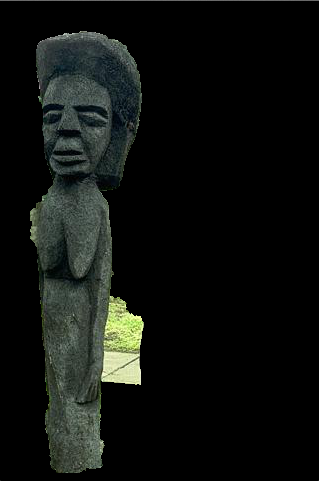
\includegraphics[scale=.3]{data/grabcut-dataset/res/pillar.png}}

\caption{Clear segmentation of this image proves hard again. When all three pillars are selected, the regions in between them also get marked as foreground. If only one is selected, parts of the background always get segmented as foreground. This might be of the greeninsh-greyish color of the pillar.}%

\end{figure}

\begin{figure}
\centering
\subfloat[][The original image]{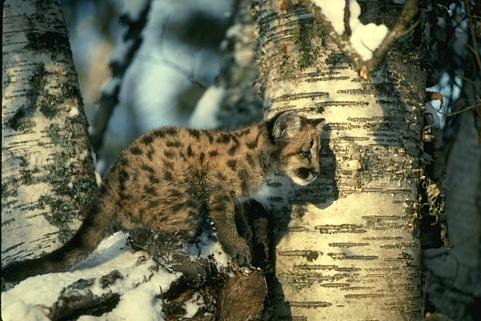
\includegraphics[scale=.5]{data/grabcut-dataset/159029.jpg}}


\caption{Segmentation of this image with the grab cut method without labeling any pixels is impossible. This is not surprising, these cats have evolved to blend into the background in order to be less visible.}%

\end{figure}

\begin{figure}
\centering
\subfloat[][The original image]{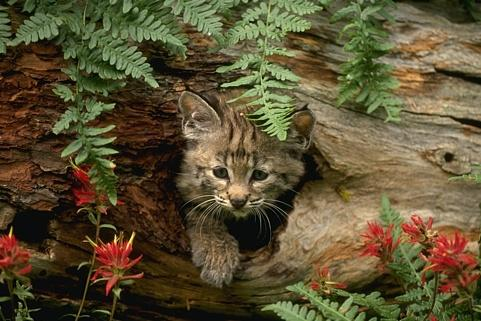
\includegraphics[scale=.3]{data/grabcut-dataset/159045.jpg}}
\quad
\subfloat[][Grab Cut]{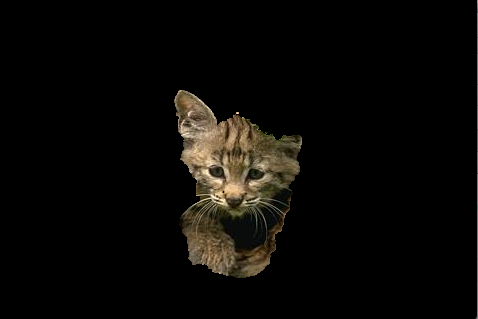
\includegraphics[scale=.3]{data/grabcut-dataset/res/cat.png}}

\caption{Clear segmentation of this image proves hard again. The kitty in the center is clearly distinguishable for us. But the fur color is similar to the bark. For the result shown in b), some additional pixels have been marked as background.}%

\end{figure}

\begin{figure}
\centering
\subfloat[][The original image]{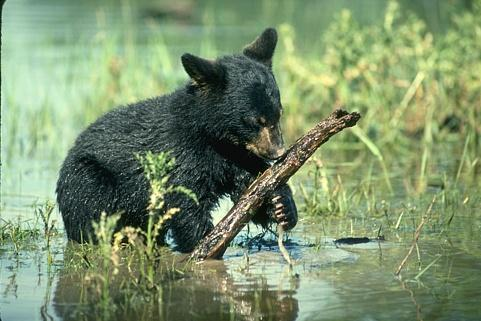
\includegraphics[scale=.3]{data/grabcut-dataset/159091.jpg}}
\quad
\subfloat[][Grab Cut]{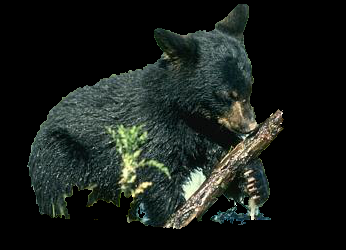
\includegraphics[scale=.3]{data/grabcut-dataset/res/bear.png}}

\caption{An acceptable segmentation of the bear is easily obtained after about 5 iterations. But the piece of grass, the log and the water seen between the legs is always included. Only seperate marking will improve segmentation (picture not shown).}%

\end{figure}

\begin{figure}
\centering
\subfloat[][The original image]{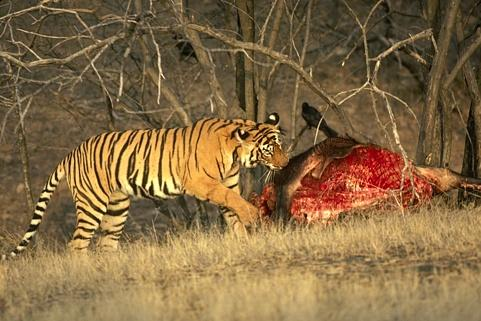
\includegraphics[scale=.3]{data/grabcut-dataset/187039.jpg}}
\quad
\subfloat[][Grab Cut]{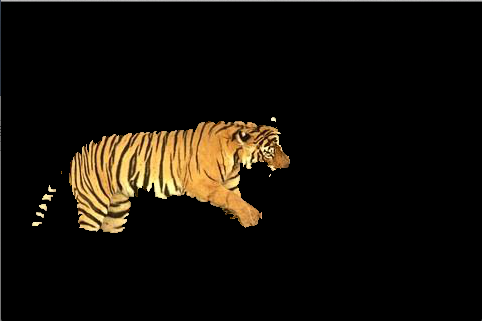
\includegraphics[scale=.3]{data/grabcut-dataset/res/tiger.png}}

\caption{The segmentation of the tiger worked better as excpeted, since it also evolved to blend in. This segmentation is obtained after 4 iterations.}%

\end{figure}

\begin{figure}
\centering
\subfloat[][The original image]{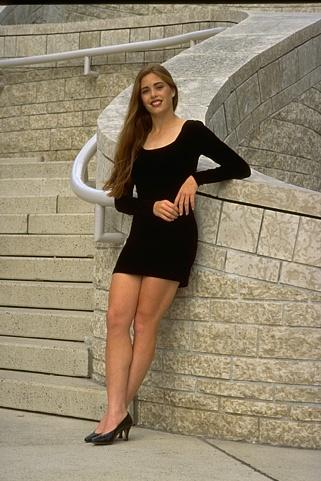
\includegraphics[scale=.3]{data/grabcut-dataset/388016.jpg}}
\quad
\subfloat[][Grab Cut]{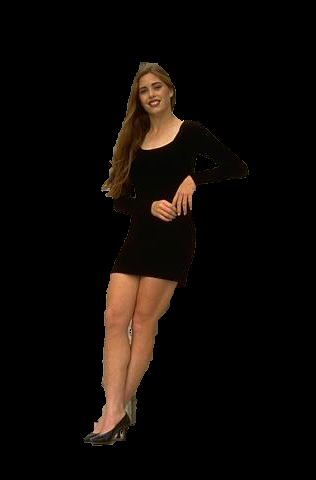
\includegraphics[scale=.3]{data/grabcut-dataset/res/woman.png}}

\caption{An acceptable segmentation of the woman is easy, it is a clear background/foreground relation.Also the dress is clearly segmented (not seen in this small picture). More difficult is a clean and smooth segmentaition of the legs. This segmenation stabilizes after 3 iterations.}%

\end{figure}
Some observations about the performance of the grab cut
\begin{itemize}
\item backgroun
\item hello
\end{itemize}



\section{Eroding and dilating}
We have made the text on the Africa map bolder by eroding with a 3 by 3 rectangle as a structuring element, as seen on Fig. \ref{fig:a2a}. We have then cleared out the text by dilating the image three times with the same rectangle structuring element as before, as seen on Fig. \ref{fig:a2a}. For the map outline, we cancelled out the text as before, then we eroded three times to revert the effects of dilation on the map outline, then we copied the image, eroded again and subtracted the copy from the image. The result can be seen in Fig. \ref{fig:a2a}.
\begin{figure}%
\centering
\subfloat[][The original image]{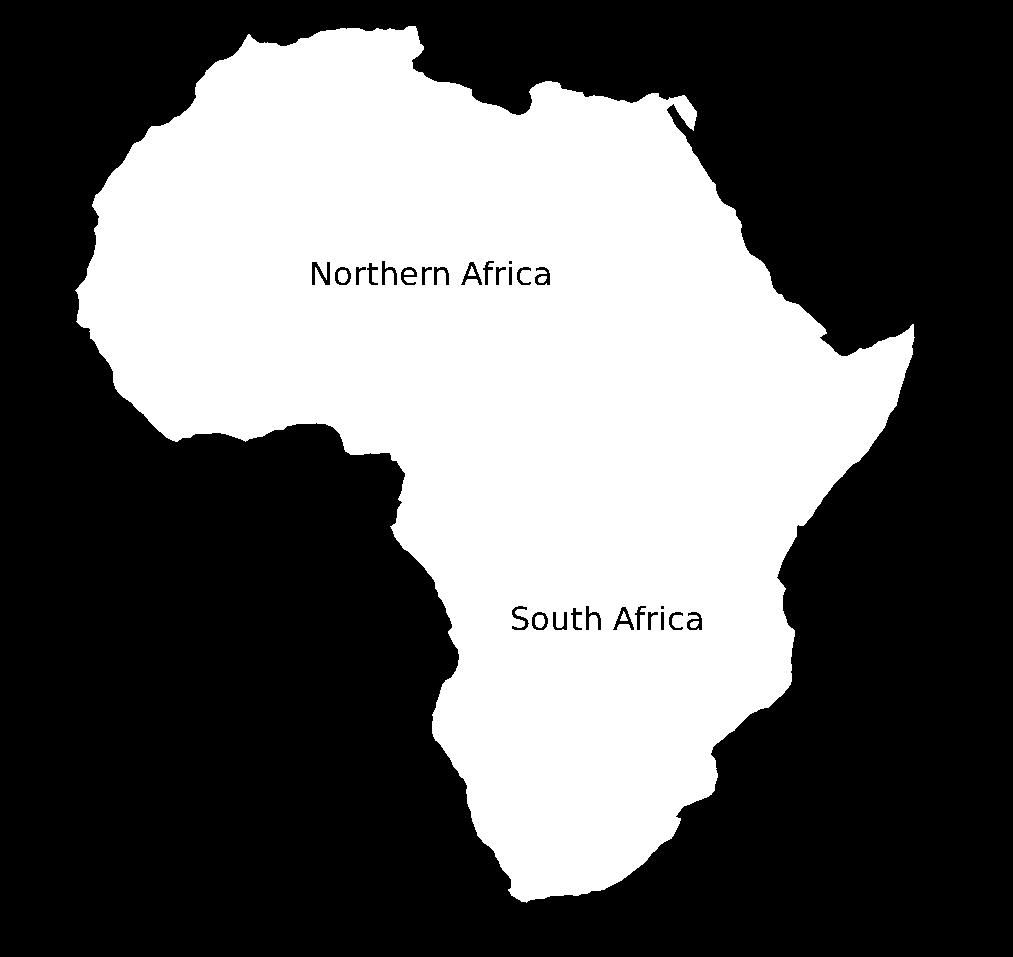
\includegraphics[scale=.3]{data/africa.png}}
\quad
\subfloat[][Eroded]{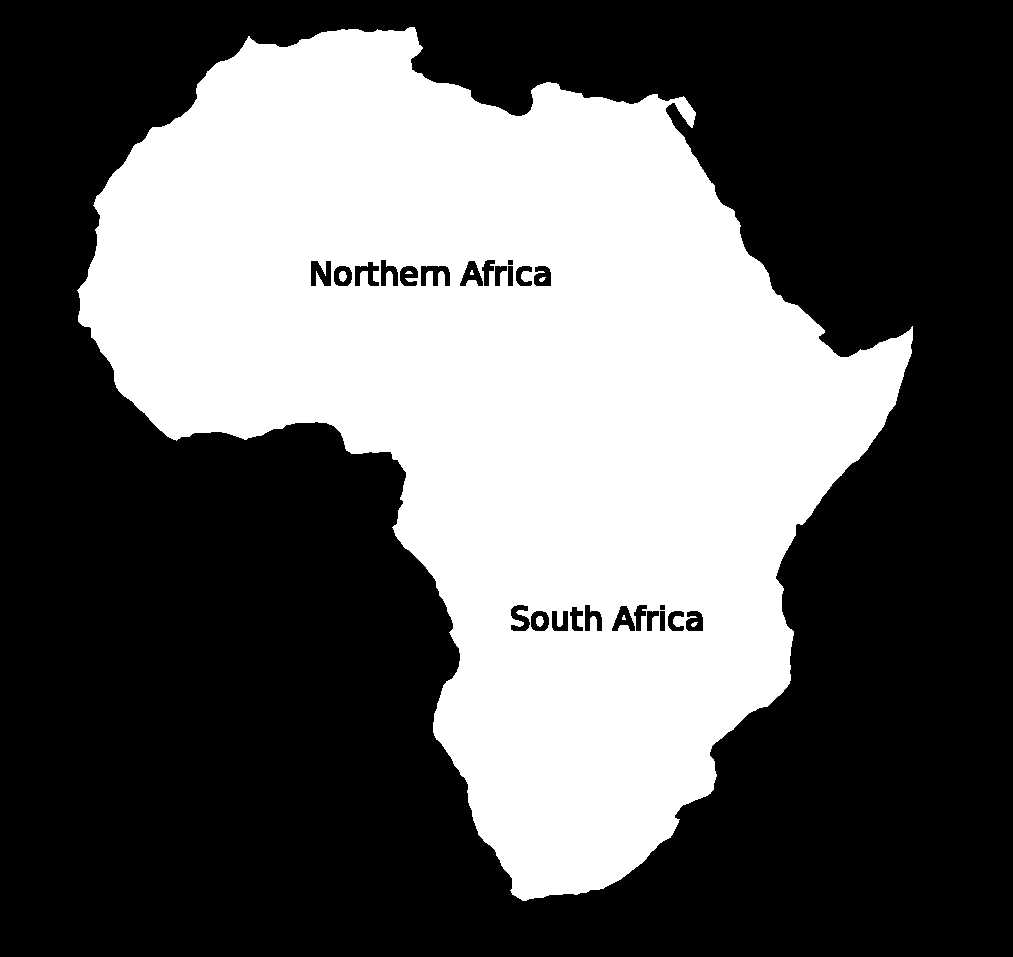
\includegraphics[scale=.3]{data/res/eroded.png}}
\quad
\subfloat[][Dilated]{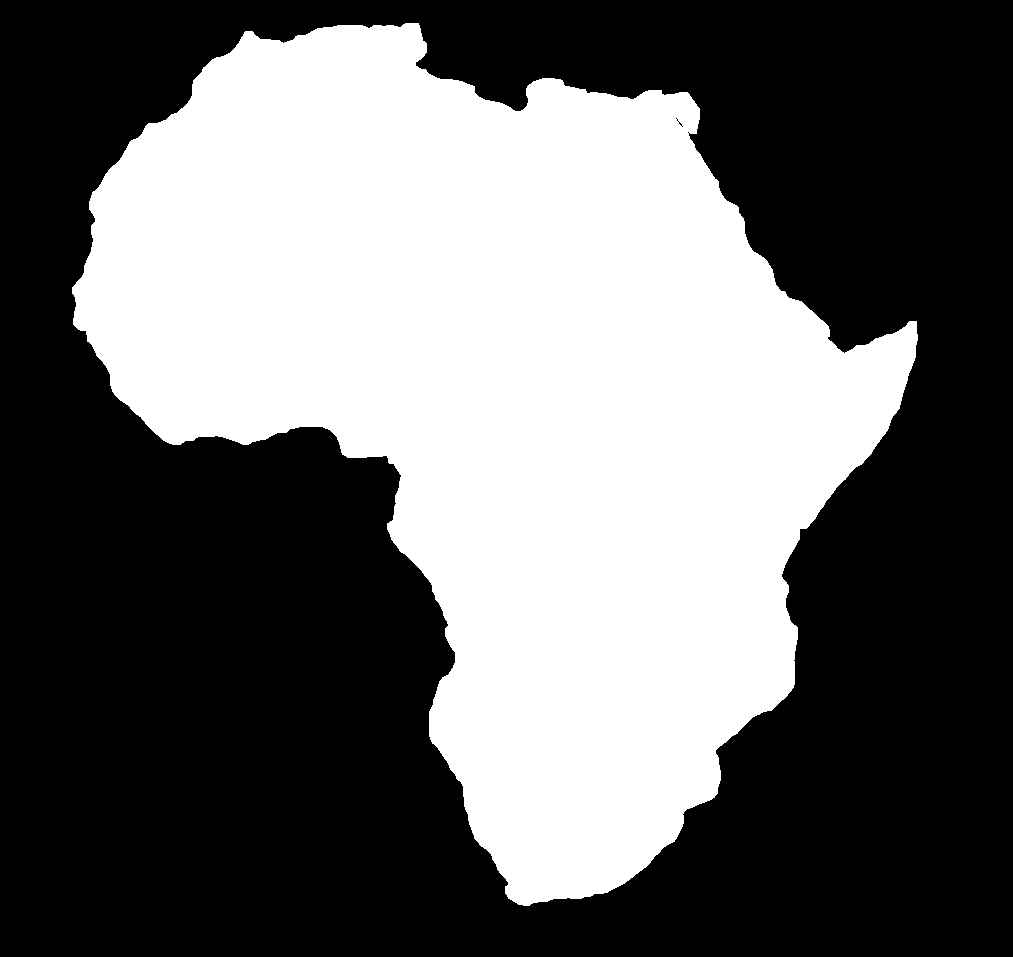
\includegraphics[scale=.3]{data/res/dilated.png}}
\quad
\subfloat[][Outlines through erosion and subtraction]{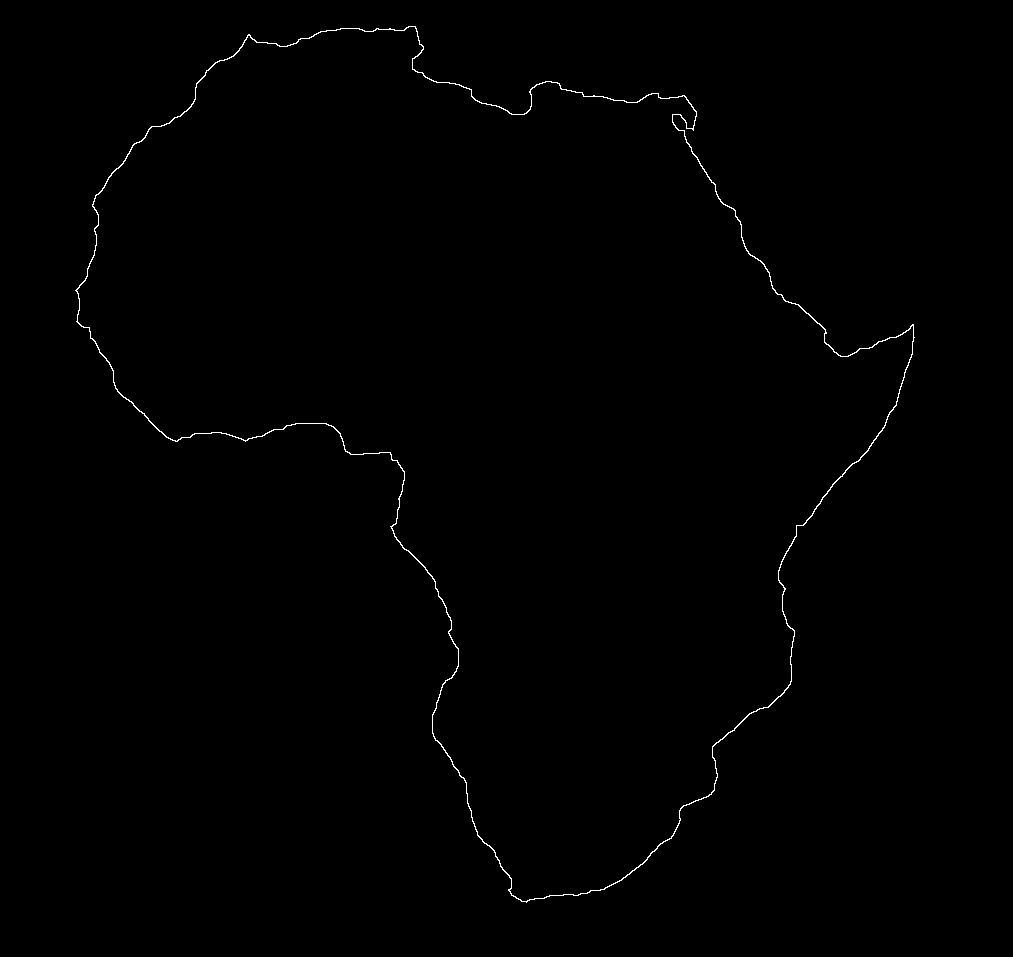
\includegraphics[scale=.3]{data/res/border.png}}
\quad
\caption{Erosion and dilation on a binary image}%
\label{fig:a2a}%
\end{figure}

\section{Opening and closing}
By using opening with a 9 by 9 circle as a structuring element, we were able to separate the dots from the lines in Fig. \ref{fig:a2b}. For the cells image, we have found that applying the same opening operation with a 7 by 7 circle after thresholding is very well suited for finding blobs above a certain size, in this case the larger cell bodies. We have also applied closing to the circles image with the same disk shaped structuring element and have discovered that this operation makes the line circles around the filled circles disappear.
Making the structuring element bigger (17 by 17) will slowly get rid of the smaller dots and in the end as it gets large enough (33 by 33) it will cancel all the dots in the image.

\begin{figure}%
\centering
\subfloat[][The original dotsandlines image]{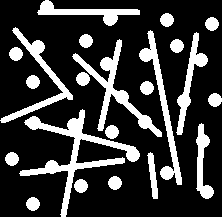
\includegraphics[scale=.3]{data/dotsandlines.png}}
\quad
\subfloat[][Separated]{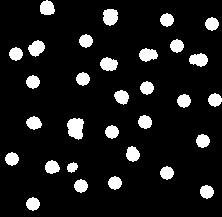
\includegraphics[scale=.3]{data/res/dots.png}}
\quad
\subfloat[][Original Cells]{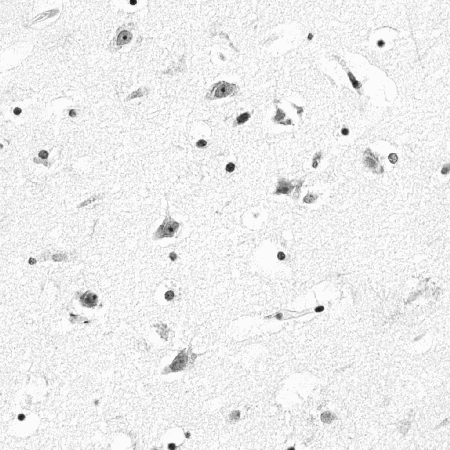
\includegraphics[scale=.3]{data/cells.png}}
\quad
\subfloat[][Thresholded Cells]{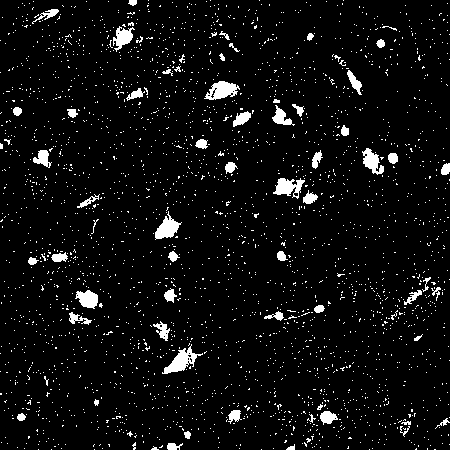
\includegraphics[scale=.3]{data/res/cells_thresh.png}}
\quad
\subfloat[][Cell body detected by opening]{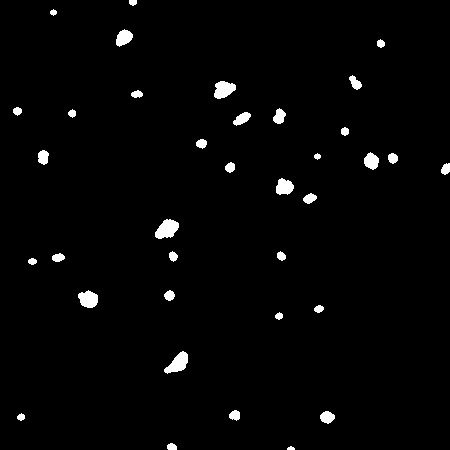
\includegraphics[scale=.3]{data/res/dots1.png}}
\quad
\subfloat[][Circles original]{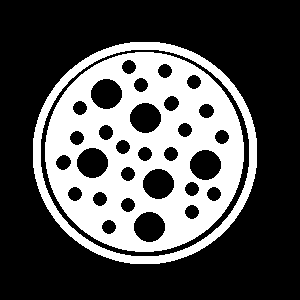
\includegraphics[scale=.3]{data/circles.png}}
\quad
\subfloat[][Circles closed]{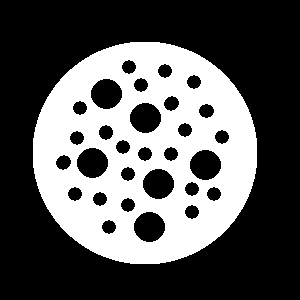
\includegraphics[scale=.3]{data/res/circles_closed9.png}}
\quad
\subfloat[][Circles closed larger element]{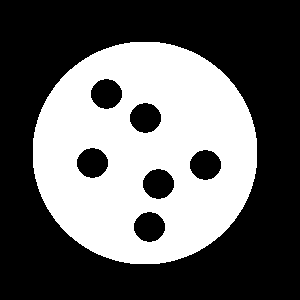
\includegraphics[scale=.3]{data/res/circles_closed17.png}}
\quad
\subfloat[][Circles closed even larger element]{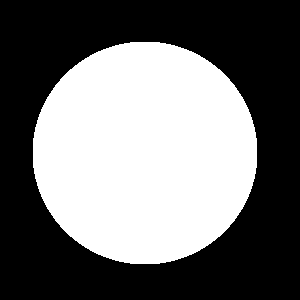
\includegraphics[scale=.3]{data/res/circles_closed33.png}}
\quad
\caption{Opening and closing}%
\label{fig:a2b}%
\end{figure}

\section{Advanced}
We have taken the house image (Fig. \ref{fig:a2c}) and tried to implement an edge detection by using the morphological gradient with a 3 by 3 cross as structuring element. After thresholding at 60, the lines are clearly visible on the output image. Compared to Canny it performs worse, since Canny also tries to suppress non-maxima and attempts to connect different parts of a line.
For corner detection, we have added the absolute value of the morphological gradient with a horizontal line as structuring element to the same with a vertical structuring element. After thresholding, regions where both gradients are strong will stay and thus we have found a corner.

\begin{figure}%
\centering
\subfloat[][The original image]{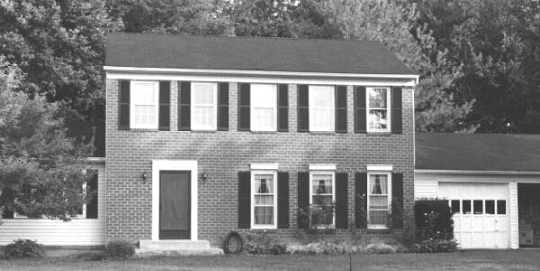
\includegraphics[scale=.3]{data/house.png}}
\quad
\subfloat[][Thresholded morphological gradient]{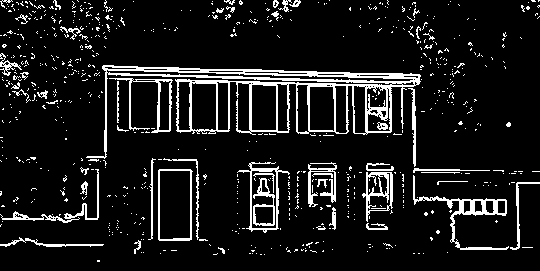
\includegraphics[scale=.3]{data/res/grad.png}}
\quad
\subfloat[][Canny]{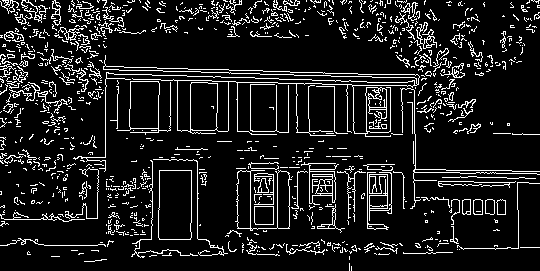
\includegraphics[scale=.3]{data/res/canny.png}}
\quad
\subfloat[][Corner detection]{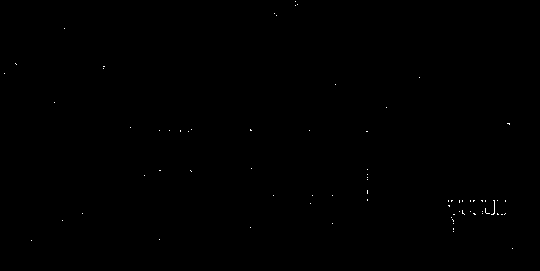
\includegraphics[scale=.3]{data/res/corners.png}}
\quad
\caption{Advanced morphological operations}%
\label{fig:a2c}%
\end{figure}

\end{document}

